\documentclass[twoside]{report}
\usepackage[utf8x]{inputenc}
\usepackage[spanish]{babel}
\usepackage{amssymb}
\usepackage{amsmath}
\usepackage{amsthm}
\usepackage{hyperref}
\hypersetup{colorlinks=true,citecolor=red, linkcolor=blue}
\usepackage{subfiles}
\usepackage[]{graphicx}
\usepackage{svg}
\setsvg{inkscape=inkscape -z -D}

\SetUnicodeOption{mathletters}
\SetUnicodeOption{autogenerated}

\renewcommand{\baselinestretch}{1,4}
\usepackage[papersize={210mm,297mm},
            twoside,
            includehead,
            top=1in,
            bottom=1in,
            inner=0.75in,
            outer=1.0in,
			bindingoffset=0.35in]{geometry}

\theoremstyle{definition}
\newtheorem{theorem}{Teorema}[section]
\newtheorem{propi}[theorem]{Propiedades}
\newtheorem{condition}{Condition}
\newtheorem{consecuencia}[theorem]{Consecuencia}
\newtheorem{observacion}[theorem]{Observación}
\newtheorem{coro}[theorem]{Corolario}
\newtheorem{defi}[theorem]{Definición}
\newtheorem{example}[theorem]{Ejemplo}
\newtheorem{lemma}[theorem]{Lema}
\newtheorem{nota}[theorem]{Nota}
\newtheorem{ejer}[theorem]{Ejercicio}
\newtheorem{prop}[theorem]{Proposición}
\newtheorem*{dem}{Demostración}
\newcommand*{\QED}{\hfill\ensuremath{\blacksquare}}

\newtheorem{summary}{Summary}
\numberwithin{equation}{section}
\newcommand{\Z}{\mathbb{Z}}
\newcommand{\R}{\mathbb{R}}
\newcommand{\X}{\mathbb{X}}
\newcommand{\seaX}{\X:U\rightarrow\R^3}
\newcommand{\luego}{\Rightarrow}
\newcommand{\sii}{\Leftrightarrow}
\newcommand{\resi}{\varepsilon_L}
\providecommand{\conv}[1]{\overset{#1}{\longrightarrow}}
\providecommand{\convcs}{\xrightarrow{CS}}
\providecommand{\supf}{\mathbb{X}}
\providecommand{\lrg}{\longrightarrow}
%--------------------------------------------------------
\begin{document}
\chapter{Geometría}
\section{Paralelismo en superficie}
Sean $\X:U\to\R^3$ s.s., $\alpha=\X(u^1(t),u^2(t))$ c.p.r. en $\X$.

\begin{defi}
Diremos que $X(t)$ es un campo vectorial tangente a lo largo de $\alpha$ si $X(t) \in T_{\alpha(t)}(\X)$. Por ejemplo, $\dot{\alpha}(t)$ o $S(t)$.
\end{defi}

\begin{defi}
Sea X(t) un c.v.t. a lo largo de $\alpha$. Se dirá que $X(t)$ es paralelo a lo largo de $\alpha$ si $X'(t) \parallel N(t)$. El parámetro t no es esencial para la definición de campo paralelo.
\end{defi}

\begin{example}
$\X(u)$ va a ser el plano euclídeo $OXY$ y $\alpha$ una curva contenida en él. Consideramos el campo vectorial $X(t)=(a(t),b(t),0)$ que es paralelo a lo largo de $\alpha$ si $X'(t)\parallel N=(0,0,1)$. Esto nos conduce a que $(a'(t),b'(t),0)\parallel (0,0,1)\Leftrightarrow a'(t)=b'(t)=0\Leftrightarrow X(t)=(a,b,0)$ constante. Vemos pues que el campo es paralelo en el sentido euclídeo.
\end{example}

\begin{example}
Consideramos la esfera $S^2$ y tomamos como curva $\alpha$ el ecuador de la misma. El campo vectorial $X(t)=(0,0,1)$ es paralelo a lo largo de $\alpha$ puesto que $X'(t)=(0,0,0)\parallel N(t)$.
\end{example}

\begin{example}
Volvamos a considerar la esfera, esta vez parametrizada como
\[ \X(\theta,\varphi)=(\cos\theta\cos\varphi,\sen\theta\cos\varphi,\sen\varphi)\quad \theta\in(0,2\pi),\varphi\in\left(-\frac{\pi}{2},\frac{\pi}{2}\right)\]
Definimos entonces la curva $\alpha(\theta)=\X(\theta,\frac{\pi}{4})=(\frac{\sqrt{2}}{2}\cos\theta,\frac{\sqrt{2}}{2}\sen\theta,\frac{\sqrt{2}}{2})$, que es un paralelo. De este modo, el vector tangente es $X(\theta)=\X_2(\theta,\frac{\pi}{4})$. Así pues, $X'(\theta)=(\frac{\sqrt{2}}{2}\sen\theta,-\frac{\sqrt{2}}{2}\cos\theta,0)$. Basta comprobar que $X'(\theta)$ no es perpendicular a $\X_2$ para comprobar que no es un campo paralelo a lo largo de $\alpha$.
\end{example}

\begin{theorem}
El c.v.t. $X(t)=\sum_{k=1}^2 X^k \X_k$ a lo largo de α es campo paralelo a lo largo de α si y sólo si:
\[ \frac{dX^k(t)}{dt} + \sum_{i,j=1}^2 Γ_{ij}^k X^i(t) \frac{du^j}{dt} = 0 \quad \forall k=1,2 \]
\end{theorem}
\begin{dem}
Derivando $X(t)$:
\begin{align*} X'(t) & = \sum_{k=1}^2 \left(\frac{dX^k(t)}{dt}\X_k + \sum_{j=1}^2 X^k(t)\X_{kj}\frac{du^j}{dt}\right) \\
 & \overset{\text{Ec. Gauss}}{=} \sum_{k=1}^2 \left(\frac{dX^k(t)}{dt}\X_k + \sum_{j=1}^2 X^k(t)\left[\sum_{i=1}^2 Γ_{kj}^i \X_i + L_{kj}N\right]\frac{du^j}{dt}\right) \\
 & = \sum_{k=1}^2 \left[ \frac{dX^k}{dt}(t) + \sum_{i,j=1}^2 Γ_{ij}^k X^i(t) \frac{du^j}{dt}\right]\X_k + \left[\sum_{i,j=1}^2 L_{ij} X^i(t) \frac{du^j}{dt}\right]N(t)
\end{align*}
Llamamos al primer sumando \textbf{parte  tangente} y al segundo sumando, \textbf{parte normal}. De aquí:
\[ X'(t) \parallel N(t) \Leftrightarrow \frac{dX^k}{dt} + \sum Γ_{ij}^k X^i(t) \frac{du^j}{dt} = 0\quad \forall k=1,2\]
$\QED$
\end{dem}

\begin{defi}
Llamamos \textbf{derivada covariante} de $X(t) = \sum_{k=1}^2 X^k \X_k$ a:
\[ \frac{DX(t)}{dt} = \sum_{k=1}^2 \left[ \frac{dX^k(t)}{dt} + \sum_{i,j=1}^2 Γ_{ij}^k X^i(t) \frac{du^j}{dt}\right]\X_k\]
\end{defi}

\begin{consecuencia}
$X(t)$ c.v.t. es paralelo a lo largo de $α$ si y sólo si $\frac{DX(t)}{dt} = 0$.
\end{consecuencia}

\begin{consecuencia}
El concepto de \emph{paralelismo} (campo paralelo) es intrínseco de la superficie. Recuérdese que lo símbolos de Christoffel son intrínsecos a la superficie, ya que:
\[ Γ_{ij}^k = \frac{1}{2} \sum_{h=1}^2 g^{hk} (g_{ih,j}+g_{jh,i}-g_{ij,h}) \]
donde $g_{xy,z} = \dfrac{\partial g_{xy}}{\partial u^z}$.
\end{consecuencia}

\begin{theorem}[Existencia y unicidad de campos paralelos]
Sea $α(t) = \X(u¹(t), u²(t))$ c.p.r. en $\X : U \to \R³$. Entonces existe un único c.v.t. $X(t)$ paralelo a lo largo de $α$ con $X(t_0)=v_0$.
\end{theorem}

\begin{dem}
Si existe $X(t) = \sum_{k=1}^2 X^k \X_k$ c.v.t. paralelo a lo largo de $α$, $X^k(t)$ cumple que:
\[ \frac{dX^k(t)}{dt} + \sum_{i,j=1}^2 Γ_{ij}^k(t) X^i(t) \frac{du^j}{dt} = 0 \quad k=1,2 \]
\[ X^1(t_0) = v_0^1  \qquad X^2(t_0) = v_0^2 \]
Estamos ante un problema de Cauchy. Por el teorema de Picard, existe solución y es única.
$\QED$
\end{dem}

\begin{defi}
El campo $X(t)$ obtenido integrando el sistema anterior y que cumple $X(t_0) = v_0$, se llama el \textbf{transporte paralelo} de $v_0$ a lo largo de $α$.
\end{defi}

%\begin{observacion}
%Dada $α(t)$ y $v_0$, el campo $X(t)$ paralelo es único, pero si el camino $α$ va de $p$ a $q$ de $X^k$ de $X(t)$ satisface las ecuaciones diferenciales de $(1.13)$
%\end{observacion}

\begin{observacion}
El transporte paralelo depende del camino.
\end{observacion}

\begin{example}
En $S^2(1)$, consideramos la curva $α(θ) = (\cos θ \cos φ_0, \sen θ \cos φ_0, \sen φ_0)$ con ${θ \in [0,2\pi]}$. Se tiene:
\[ \X_1 = (- \sen θ \cos φ, \cos u \cos φ, 0) \]
\[ \X_2 = (- \cos θ \sen φ, - \sen θ \sen φ, \cos φ) \]
\[ g_{11} = \cos²φ \qquad g_{12} = 0 \qquad g_{22} = 1 \]
\[ Γ_{12}^1 = - \tan φ \qquad Γ_{11}^2 = \cos φ \sen φ \]
\[ u¹ = θ, u² = φ \]

Para que $X(θ) = X^1(θ) \X_1(θ,φ_0) + X^2 \X_2(θ, φ_0)$ sea c.v.t. paralelo, se debe cumplir que:
\[ \frac{dX^1}{dθ} - \tan φ_0 X^2 = 0 \]
\[ \frac{dX^2}{dθ} + \cos φ_0 \sen φ_0 X^1 = 0 \]
De ahí se obtiene integrando que:
\[ X^1(θ) = \frac{1}{\cos φ_0} \sen ( θ \sen φ_0) \]
\[ X^2(θ) = \cos(θ \sen φ_0) \]
Luego:
\[ X(θ) = \frac{1}{\cos φ_0} \sen (θ \sen φ_0) \X_1 - \cos (θ \sen φ_0) \X_2 \]
Sin embargo, $X(0) = \X_2(0,φ_0) \neq X(2\pi) = \frac{1}{\cos φ_0}\sen (2\pi \sen φ_0) \X_1 - \cos (2 \pi \sen φ_0) \X_2$. El transporte paralelo del vector $X(0)$ no va a mantener siempre constante el vector al pasar la curva por el mismo punto.
\end{example}
\begin{prop}
Sean $X(t),Y(t)$ c.v.t. paralelos a lo largo de una curva $α(t) = \X(u¹(t), u²(t))$. Entonces el transporte paralelo de vectores a lo largo de $\alpha$ conserva módulos y ángulos.
\end{prop}
\begin{dem}
Consideramos el producto escalar $X(t)\cdot Y(t)$. Derivando respecto de t y teniendo en cuenta que $X'(t) \parallel Y'(t) \parallel N(t)$:
\[
(X(t)\cdot Y(t))' = X'(t)\cdot Y(t) + X(t) \cdot Y'(t) = 0
\]
Como el producto escalar es constante, el módulo $\sqrt{X(t)\cdot X(t)}$ también lo ha de ser. Además, para el ángulo se tiene:
\[
\cos{\varphi(t)}=\frac{X(t)\cdot Y(t)}{|X(t)||Y(t)|} = cte
\]
\end{dem}
\begin{consecuencia}
Si tenemos una superficie $M$ parametrizada como $\X(u^1,u^2)$ y una curva $α(t) = \X(u¹(t), u²(t))$, $P\in \alpha$ y dos $v_1,v_2$ que son base de $T_P(\X)$. Entonces, si trasladamos dichos vectores mediante un transporte paralelo a Q, estos mantendrán el ángulo y sus respectivos módulos. Si tomamos $v_1$ y $v_2$ ortonormales, su transporte paralelo forma también una base ortonormal en Q. Esto se denomina \textbf{conexión de la geometría de la superficie M en P y Q}.
\end{consecuencia}
\begin{defi} Sea $α(t) = \X(u¹(t), u²(t))$ c.p.r. en $\X : U \to \R³$. Se llama \textbf{autoparalela} si el c.v.t. $\alpha'(t)$ es un campo paralelo a lo largo de $\alpha$.
\end{defi}
\begin{prop}
Una curva $\alpha(t)$ es autoparalela si y solo si es geodésica y $t$ es función lineal del parámetro natural.
\end{prop}
\begin{dem}
$(\Rightarrow)$ Supongamos que $\alpha$ es autoparalela. Por ser c.v.t. paralelo,  $|\alpha'(t)| = cte = a$, por tanto $s=\int_{t_0}^t|\alpha'(x)|dx = at+b$. Además:
\[
\alpha' = \dot{\alpha} \frac{ds}{dt} =\dot{\alpha}a \qquad
 \alpha''  = \ddot{\alpha}a^2
 \]
Como $\alpha'' \parallel N$, entonces $\ddot{\alpha}=k(s)n(s)\parallel N$. Por tanto, $\alpha$ es geodésica.\\
$(\Leftarrow)$ Supongamos que $\alpha(t)$ es geodésica y que $t=as+b$. Entonces
\begin{gather*}
\alpha'(t)=\frac{d\alpha(s)}{ds}\frac{ds}{dt}=\dot{\alpha}(s)\frac{1}{a}\\
\alpha''(t)=\ddot{\alpha}(s)\frac{1}{a^2}=k(s)n(s)\frac{1}{a^2}
\end{gather*}
Como $\alpha$ es geodésica, $n\parallel N$, luego $\alpha''(t)\parallel N$, de modo que $\alpha'(t)$ es c.v.t. paralelo y por ende $\alpha$ es autoparalela.
\end{dem}

\begin{nota}
Sea $X(s)$ c.v.t. paralelo unitario a lo largo de $\alpha$. Sea $\varphi(s)=\widehat{(X(s),\dot{\alpha}(s))}$ entonces:
\begin{align*}
\cos{\varphi(s)}&=X(s)\dot{\alpha}(s)\\
 -\dot{\varphi}(s)\sin\varphi(s)& =  X'(s)\dot{\alpha}(s)+ X(s)\ddot{\alpha}(s)= X(s)(K_g(s)S(s)+K_n(s)N(s))=K_g(s)X(s)S(s)\\
  &= K_g(s)|X(s)||S(s)|cos{(\varphi+\frac{\pi}{2})}=-K_g\sin{\varphi}
\end{align*}
Luego $K_g = \dot{\varphi}$, similar a la curvatura plana.
\end{nota}
\begin{example}
Consideramos $S^2(1)$ y, sobre ella, $\alpha,\beta$ círculos máximos de polo norte (N) a polo sur (S). Por ser círculos máximos, $\alpha,\beta$ son geodésicas. Sea $X\in T_N(S^1)$ tangente a $\alpha$. Si realizamos un transporte paralelo de X hasta S por $\alpha$ usando $\dot{\alpha}$, obtenemos un vector $X_\alpha$ tangente a $\alpha$ en S. Sea $Y\in T_N(S^1)$ tangente a $\beta$ obteniendo, análogamente, $Y_\beta$. Sea $\theta=\widehat{\alpha,\beta}$. En el polo norte $\theta=\widehat{X,Y}$. Como $\dot{\beta}$ es un c.v.t. paralelo a $\beta$, podemos transportar $X$ a lo largo de $\beta$, obteniendo un vector $X_\beta$. Como $X$ y $\dot{\beta}$ mantienen sus ángulos, se tiene que $\widehat{X_\alpha,X_\beta}=2\theta$. Curiosiamente: $2\theta=A(R)$, donde R es la región esférica que delimitan $\alpha$ y $\beta$.
\end{example}
\begin{propi}
Sean $X(t),Y(t)$ c.v.t. a lo largo de $\alpha(t)$. Se tiene:
\begin{itemize}
\item La derivada covariante es un operador lineal.
\item $\dfrac{D(f(t)X(t))}{dt} = X(t)f'(t)+\dfrac{DX(t)}{dt}f(t)$.
\item $(X(t)\cdot Y(t))' = X'(t)Y(t)+X(t)Y'(t) = \dfrac{DX(t)}{dt}Y(t)+X(t)\dfrac{DY(t)}{dt}$.
\end{itemize}
\end{propi}


\section{La curvatura geodésica de una curva en una superficie}

\begin{prop}
Dada $\X : U \to \R^3$ s.s., existe un cambio de parámetro regular de forma que las líneas paramétricas de los nuevos parámetros son ortogonales (es decir, $\overline{g}_{12}=0$).
%Dibujo: Cambio de variable
\end{prop}

\begin{dem}
Empezamos buscando una curva $β(σ)=\X(u¹(σ),u²(σ))$ tal que sea ortogonal a las $u²$-paramétricas. Se tiene que el vector tangente a $β$ es:
\[ β'(σ) = \X_1 \frac{du¹}{dσ}+\X_2 \frac{du²}{dσ} \]
Para que $β'(σ) \cdot \X_2 = 0$:
\[ β'(σ) \cdot \X_2 = g_{12} \frac{du¹}{dσ} + g_{22} \frac{du²}{dσ} = 0 \]
El problema se reduce a integrar la 1-forma:
\[ g_{12} du¹ + g_{22} du² = 0 \]
Existe un factor integrante $μ(u¹,u²)\neq 0$ tal que $μ g_{12} du¹+μ g_{22} du² = dh(u¹,u²)= du¹+h_2 du²$ para algún $h$. Necesariamente $μ g_{12} = h_1$ y $μ g_{22} = h_2$. Sea el cambio de parámetros:
\[ f^{-1} = \begin{cases}
	\overline{u}¹ = u¹\\
	\overline{u}² = h(u¹,u²)
\end{cases}\]
El cambio de parámetros está bien definido ya que $f^{-1} \in \mathcal{C}^\infty$ y $|J(f^{-1})| = \begin{vmatrix}1 & 0\\h_1 & h_2\end{vmatrix} = h_2 = μ g_{22} \neq 0$. Luego:
\[ \overline{g}_{ij} = \sum g_{hk} \frac{du^h}{d\overline{u}^i} \frac{du^k}{d\overline{u}^j}\]
En particular:
\[ \overline{g}_{12} = \sum g_{hk} \frac{du^h}{d\overline{u}^1} \frac{du^k}{d\overline{u}^2} \]
Como $J(f^{-1}) = \begin{pmatrix}1 & 0\\h_1 & h_2\end{pmatrix} = \begin{pmatrix}1 & 0\\μ g_{12} & μ g_{22}\end{pmatrix}$, $J(f) = (J(f^{-1})^t)^{-1} = \begin{pmatrix}1 & 0 \\ -\frac{g_{12}}{g_{22}} & \frac{1}{μg_{22}}\end{pmatrix} = \begin{pmatrix}\frac{du¹}{d\overline{u}^1} & \frac{du^1}{d\overline{u}^2}\\\frac{du^2}{d\overline{u}^1} & \frac{du^2}{d\overline{u}^2}\end{pmatrix}$
\begin{align*}
	\overline{g}_{12} & = g_{11} \frac{du¹}{d\overline{u}¹} \frac{du¹}{d\overline{u}²} + g_{12} \frac{du¹}{d\overline{u}¹} \frac{du²}{d\overline{u}} + g_{21} \frac{du²}{d\overline{u}¹} \frac{du¹}{d\overline{u}²} + g_{22} \frac{du²}{d\overline{u}¹} \frac{du²}{d\overline{u}²} \\
	& = g_{11} \cdot 1 \cdot 0 + g_{12} \cdot 1 \cdot \left(\frac{1}{µ g_{22}}\right) + g_{21} \cdot \left( \frac{-g_{12}}{g_{22}}\right) \cdot 0  + g_{22} \left(\frac{-g_{12}}{g_{22}}\right) \frac{1}{μ g_{12}} \\
	& = \frac{1}{μ} - \frac{1}{μ} = 0
\end{align*}
\qed
\end{dem}
Buscamos una fórmula para $K_g(s)$. Podemos suponer ya que las líneas paramétricas son ortogonales ($g_{12} = 0$). Sea $e_1(s) = \frac{\X_1}{|\X_1|} = \frac{\X_1}{\sqrt{g_{11}}}$ y $e_2(s) = \frac{\X_2}{|\X_2|} = \frac{\X_2}{\sqrt{g_{22}}}$ de manera que $\{e_1(s), e_2(s)\}$ es una base ortonormal sobre la curva $α(s)$. Sea $θ(s) = (\widehat{e_1(s), \dot{α}(s))}$. Luego:
\[ \dot{α} = \cos θ e_1 + \sen θ e_2 \]
\[ S = - \sen θ e_1 + \cos θ e_2\]

Obtenemos la derivada covariante de $\dot{α}$:
\begin{align*}
	\frac{D\dot{α}}{ds} & = tg\left(\frac{d\dot{α}}{ds}\right) = tg(-\sen{θ} \dot{θ} e_1 + \cos{θ} \dot e_1 + \cos θ \dot{θ} e_2 + \sen θ \dot e_2) \\
	& = - \sen θ \dot{θ} e_1 + \cos θ \frac{D e_1}{ds} + \cos θ \dot{θ} e_2 + \sen θ \frac{De_2}{ds}\\
	\frac{de_1}{ds} & = \dot{e}_1 = \frac{d}{ds}\left(\frac{\X_1}{\sqrt{g_{11}}}\right) = \frac{d}{ds} \frac{1}{\sqrt{g_{11}}} \X_1 + \frac{1}{\sqrt{g_{11}}} \left(\X_{11} \frac{du¹}{ds} + \X_{12} \frac{du²}{ds}\right)
\end{align*}
Como $e_1(s) \cdot e_2(s) = 0$, luego $\dot{e}_1 \cdot e_2 = -e_1 \cdot \dot{e}_2$. Sea $w(s) = \dot{e_1}\cdot e_2$
\[ \frac{d}{ds} (e_i \cdot e_i) = 0 = 2 \dot{e}_i \cdot e_i \Rightarrow \dot{e}_i \perp e_i \]
\begin{equation} \frac{de_i}{ds} \cdot e_i = 0 \Rightarrow \frac{D e_i}{ds} \cdot e_i = 0 \Rightarrow \frac{De_i}{ds} \parallel e_j \text{ con } j \neq i \end{equation}
Por lo tanto:
\[ \frac{De_1}{ds} \cdot e_2 = \frac{de_1}{ds} \cdot e_2 = \dot{e}_1 \cdot e_2 = w(s)\]
Análogamente, $\frac{De_2}{ds} \cdot e_1 = -w(s)$. Usando además que (1.2.1):
\[ \frac{De_1}{ds} = w e_2 \]
\[ \frac{De_2}{ds} = -w e_1\]
Finalmente:
\begin{align*}
	\frac{D\dot{α}}{ds} & = -\sen θ \dot{θ} e_1 + \cos θ w e_2 + \cos θ \dot{θ} e_2 + \sen θ (-w) e_1 \\
	& = (-\dot{θ} -w) \sen θ e_1 + (\dot{θ} + w) \cos θ e_2 = (-\sen θ e_1 + \cos θ e_2) (\dot{θ}  w) = (\dot{θ} + w)\cdot S
\end{align*}


\begin{theorem}
Se $θ(s) = (\widehat{\X_1(s), \dot{α}(s))}$. En las condiciones anteriores se tiene:
\[ K_g(s) = \dot{θ}(s) + \frac{1}{2 \sqrt{g_{11}g_{22}}} \left((g_{22})_1 \dot{u}²(s) - (g_{11})_2 \dot{u}¹(s) \right)\]
\end{theorem}

\begin{dem}
\[ \ddot{α}(s) = k(s)n(s) = K_g \cdot S + K_n \cdot N \]
Multiplicando por $S$:
\[ \ddot{α}(s) \cdot S = K_g \Rightarrow K_g = tg\left(\frac{d\dot{α}}{ds}\right) \cdot S = \frac{D\dot{α}}{ds} \cdot S = \dot{θ} + w \]
\end{dem}

Calculamos $w=\dot{e}_1 \cdot e_2$:
\[ \dot{e}_1 = \left(\frac{\X_1}{\sqrt{g_{11}}}\right)' = \frac{d}{ds} \left(\frac{1}{\sqrt{g_{11}}}\right) \X_1 + \frac{1}{\sqrt{g_{11}}} (\X_{11} \cdot \dot{u}^1 + \X_{12} \dot{u}²) \]
Por otro lado:
\[ 0 = g_{12} = \X_1 \cdot \X_2 \Rightarrow 0 = \X_{11} \X_2 + \X_1 \X_{12} \Rightarrow \X_{11} \cdot \X_2 = - \X_1 \cdot \X_{12} \]
\[ g_{11} = \X_1 \cdot \X_1 \Rightarrow 2 \X_1 \cdot \X_{12} = (g_{11})_2 \]
Usando las dos igualdades: $\X_{11}\cdot \X_2 = \dfrac{-(g_{11})_2}{2}$. Análogamente:
\[ g_{22} = \X_2 \cdot \X_2 \Rightarrow 2 \X_{12} \cdot \X_2 = (g_{22})_1 \]
Luego
\begin{align*} 
ω(s) & = \dot{e}_1 \cdot e_2 = \left[\frac{d}{ds} (\frac{1}{\sqrt{g_{11}}}) \X_1 + \frac{1}{\sqrt{g_{11}}} (\X_{11} \cdot \dot{u}^1 + \X_{12} \dot{u}²)\right] \cdot e_2 \\
	& = \left(\frac{1}{\sqrt{g_{11}}}\right)' \X_1 \cdot e_2 + \frac{1}{\sqrt{g_{22}}\sqrt{g_{11}}} (\X_{11} \dot{u}¹+ \X_{12} \dot{u}²) \cdot \X_2 = \frac{1}{\sqrt{g_{11} g_{22}}}
	\left[(\X_{11} \cdot \X_2)  \dot{u}^1 + (\X_{12} \cdot \X_2) \dot{u}²\right] \\
	& = \frac{1}{2 \sqrt{g_{11}g_{22}}} \left((g_{22})_1 \dot{u}²(s) - (g_{11})_2 \dot{u}¹(s) \right)
\end{align*}
\newpage
\section{Curvas diferenciables por arcos en una s.s.}
\begin{defi} 
Sea $\alpha:[0,L] \rightarrow \R^3$ una curva en $\X:U\rightarrow \R^3$. Se dice que es regular por arcos si existe una partición finita $0=s_1 < s_2 < \dotsc < s_{n+1} = L$ de forma que $\alpha_{|_{(s_i,s_{i+1})}}$ es regular. Los $\alpha(s_i)$ se denominan vértices y los $\alpha([s_i,s_{i+1}])$ lados.
\end{defi}
\begin{defi}
Como $\alpha$ es regular a trozos, existe el vector tangente $\alpha(s_i)$ por la izquierda $\dot{\alpha}(s_i^-)$ y por la derecha $\dot{\alpha}(s_i^+)$. Al ángulo $\varphi_i = \langle \dot{\alpha}(s_i^-),\dot{\alpha}(s_i^+)\rangle$ lo denominamos salto de la tangente en $\alpha(s_i)$.

\begin{figure}[h!]
	\centering
	\includegraphics[scale=0.4]{normal}
\end{figure}\

\end{defi}
\begin{prop}
Si $\alpha(s_i)$ es un punto singular entonces su salto $\varphi_i$ verifica que $0<|\varphi_i|\leq \pi$. Distinguimos los casos:
\begin{itemize}
\item $|\varphi_i|\neq \pi$. Tomando el sentido de giro dado por el vector normal podemos ver el signo del ángulo.
\item $|\varphi_i| = \pi$. En principio no podemos determinar si escoger $\pi$ o $-\pi$. Para ello tomamos el vector tangente en $\dot{\alpha}(s_i\pm\varepsilon)$ y, se demuestra que, $\exists \varepsilon >0$ de forma que $(\dot{\alpha}(s_i -\varepsilon) \dot{\alpha}(s_i+\varepsilon) N)$ es independiente de $\varepsilon$. Por tanto, tomamos $\pi$ si el producto mixto es positivo y recíprocamente.
\end{itemize}
\end{prop}
\begin{dem}
La idea de la demostración es desarrollar en serie el producto mixto. Dado que:
\begin{align*}
\dot{\alpha}(s_i-\varepsilon) = & \dot{\alpha}(s_i^-) - \ddot{\alpha}(s_i^-)\varepsilon + \dddot{\alpha}(s_i^-)\varepsilon^2 + \dotsc\\
\dot{\alpha}(s_i+\varepsilon) = & \dot{\alpha}(s_i^+) + \ddot{\alpha}(s_i^+)\varepsilon + \dddot{\alpha}(s_i^+)\varepsilon^2 + \dotsc
\end{align*}
\begin{gather*}
(\dot{\alpha}(s_i -\varepsilon) \dot{\alpha}(s_i+\varepsilon) N) = (\dot{\alpha}(s_i^-) \dot{\alpha}(s_i^+)  N) + \varepsilon (\dot{\alpha}(s_i^-) \ddot{\alpha}(s_i^+)  N) - \varepsilon(\ddot{\alpha}(s_i^-) \dot{\alpha}(s_i^+)  N) + \frac{\varepsilon^2}{2}(\dotsc) \approx\\
\varepsilon[(t^- \dot{t}^+N) + (t^+\dot{t}^-N)] = \varepsilon(t^-,\dot{t}^+ - \dot{t}^- , N)
\end{gather*}
\end{dem}
\begin{defi}
Sea $\X:U\rightarrow\R^3$, si $U$ es homeomorfo a un disco abierto de $\R^2$ la s.s. $\X$ se llama de tipo disco. Para toda s.s. alrededor de cualquier $p\in\X(U)$ existe un entorno de tipo disco.
\end{defi}
\begin{theorem}[Teorema del índice de Hopf] Sea $\alpha:[0,L]\rightarrow\R^3$ una curva cerrada, simple y regular por arcos. Entonces:
\[
\sum_i [\theta_i(s_{i+1})-\theta_i(s_i)] + \sum_i \varphi_i = \pm 2\pi
\]
donde $\theta_i(s) =\widehat{(\dot{\alpha}(s),\mathbb{X}_1)}$ a lo largo del lado $\alpha([s_i,s_{i+1}])$ y el signo depende del sentido de giro. 
\end{theorem}
\begin{defi}
Sea $\seaX$, s.s. tipo disco. Diremos que $R \subset \X(U)$ es una región \textbf{simple} si es homeomorfa a un disco cerrado y $\partial R$ es una curva cerrada simple y regular a trozos.
\end{defi}
\begin{defi}
Diremos que R está bien (positivamente) orientada si el vector normal intrínseca de la curva frontera $S(s)$ apunta al interior de la región. Más formalmente, si tomamos una curva de $\X$ que pase por un punto de la frontera y tenga como vector tangente a $S(s)$, o cuyo vector tangente forme con $S(s)$ un ángulo menor que $\pi/2$, esté dentro de la superificie.
\end{defi}



\begin{theorem}[Teorema Gauss-Bonnet Local]\label{local}
Sea $\seaX$ s.s. tipo disco, y que sea normalizada ($g_{12} \equiv 0$). Sea $R\subset \X(U)$ una región simple y $\alpha:[0,L]\rightarrow\R^3$ el borde de la región.
\[
\sum_i \int_{s_i}^{s_{i+1}} K_g(s)ds + \iint_{R} KdA +  \sum_i \varphi_i  = \pm 2\pi
\]
\end{theorem}
\begin{dem}
Sabemos que:
\begin{gather*}
K_g = \dfrac{1}{2\sqrt{g_{11}g_{22}}}\left[(g_{22})_1\dfrac{du^2}{ds}-(g_{11})_2 \dfrac{du^1}{ds}\right]+\dfrac{d\theta_i}{ds} \qquad \theta_i = \langle\dot{\alpha}(s),\X_1\rangle \\ \\
\sum_{i=0}^n  \int_{s_i}^{s_{i+1}} K_g(s) ds = \sum_{i=0}^n  \int_{s_i}^{s_{i+1}} \dfrac{1}{2\sqrt{g_{11}g_{22}}}\left[(g_{22})_1\dfrac{du^2}{ds}-(g_{11})_2 \dfrac{du^1}{ds}\right]ds + \sum_{i=0}^n  \int_{s_i}^{s_{i+1}} \dfrac{d\theta_i}{ds} ds \overset{Green}{=}\\
= \iint_{\X^{-1}(R)} \left(\frac{\frac{\partial g_{11}}{\partial u^2}}{2\sqrt{g_{11}g_{22}}}\right)_2 + \left( \frac{\frac{\partial g_{22}}{\partial u^1}}{2\sqrt{g_{11}g_{22}}} \right)_1  du^1du^2 + 2\pi - \sum_i \varphi_i 
\end{gather*}
\end{dem}


\begin{theorem}[Teorema Egregium de Gauss]
$K$ es intrínseca.
\end{theorem}
\begin{dem}
Dado que:
\[ K = \frac{L_{11}L_{22} - L_{12}^2}{g_{11}g_{22} - g_{12}^2} \luego gK = L_{11}L_{22} - L_{12}^2 \]
Recordemos que:
\[ |\X_1 \times \X_2| = \sqrt{(\X_1 \times \X_2)(\X_1 \times \X_2)} = \sqrt{(\X_1 \X_1)(\X_2 \X_2) - (\X_1 \X_2)(\X_2 \X_1)} = \sqrt{g} \]
Luego:
\[ L_{ij} = \X_{ij} \cdot N = \X_{ij} \cdot \frac{\X_1 \times \X_2}{|\X_1 \times \X_2|} = \frac{1}{\sqrt{g}} (\X_{ij} \ \X_1\ \X_2) \]
Entonces:
\begin{align}
K g & =  \frac{1}{g} [(\X_{11}\ \X_1\ \X_2)(\X_{22}\ \X_1\ \X_2) - (\X_{12}\ \X_1\ \X_2)(\X_{12}\ \X_1\ \X_2)]\nonumber\\
K g^2 & = 
\begin{vmatrix}
	\X_{11} \X_{22} & \X_{11} \X_1 & \X_{11} \X_2\\
	\X_1 \X_{22} & g_{11} & g_{12}\\
	\X_2 \X_{22} & g_{21} & g_{22}
\end{vmatrix} -
\begin{vmatrix}
	\X_{12} \X_{12} & \X_{12} \X_1 & \X_{12} \X_2\\
	\X_1 \X_{12} & g_{11} & g_{12}\\
	\X_2 \X_{12} & g_{21} & g_{22}
\end{vmatrix}\nonumber\\
& = (\X_{11} \X_{22}) g +
\begin{vmatrix}
	0 & \X_{11} \X_1 & \X_{11} \X_2\\
	\X_1 \X_{22} & g_{11} & g_{12}\\
	\X_2 \X_{22} & g_{21} & g_{22}
\end{vmatrix} - (\X_{12}\X_{12})g -
\begin{vmatrix}
	0 & \X_{12} \X_1 & \X_{12} \X_2\\
	\X_1 \X_{12} & g_{11} & g_{12}\\
	\X_2 \X_{12} & g_{21} & g_{22}
\end{vmatrix}\nonumber\\
& = (\X_{11} \X_{22} - \X_{12} \X_{12})g + \begin{vmatrix}
	0 & \X_{11} \X_1 & \X_{11} \X_2\\
	\X_1 \X_{22} & g_{11} & g_{12}\\
	\X_2 \X_{22} & g_{21} & g_{22}
\end{vmatrix}-
\begin{vmatrix}
	0 & \X_{12} \X_1 & \X_{12} \X_2\\
	\X_1 \X_{12} & g_{11} & g_{12}\\
	\X_2 \X_{12} & g_{21} & g_{22}
\end{vmatrix}\label{Kgecuacion}
\end{align}
Vemos que como $\X_i \X_i = g_{ii}$, derivando parcialmente obtenemos que $(g_{ii})_k = \X_{ik}\X_i + \X_i\X_{ik} = 2\X_{ik}\X_i$. Luego los productos de la forma $\X_{ik}\X_i$ son intrínsecos. Además, derivando $\X_1\X_2 = g_{12}$ respecto a la primera componente, tenemos que $\X_{11}\X_2 + \X_1 \X_{12} = (g_{12})_1$. Como $\X_1\X_{12}$ es intrínseco, $\X_{11}\X_2$ es intrínseco. Análogamente, $\X_{22}\X_1 + \X_1 \X_{12} = (g_{12})_2$ y $\X_{22}\X_1$ es intrínseco. Por último, derivando $\X_{12}\X_2=\frac{1}{2}(g_{22})_1$ respecto $u^1$ obtenemos que 
\[\X_{112}\X_2 + \X_{12}\X_{12} = \frac{1}{2}(g_{22})_{11}\]
Análogamente, derivando $\X_{11} \X_2 = (g_{12})_1 - \frac{1}{2}(g_{11})_2$ respecto a $u^2$:
\[ \X_{112}\X_2 + \X_{11}\X_{22} = (g_{12})_{12} - \frac{1}{2}(g_{11})_{22}\]
Restando las dos anteriores ecuaciones, obtenemos que:
\[ \X_{11} \X_{22} - \X_{12}\X_{12} = (g_{12})_{12} - \frac{1}{2} (g_{11})_{22} - \frac{1}{2} (g_{22})_{11} \]
Entonces todos los sumandos de $Kg^2$ en $\eqref{Kgecuacion}$ son intrínsecos, luego $K$ es intrínseco.
\end{dem}

\section{Triangulaciones de una superficie}
Sea $M \subseteq \R^3$ una superficie regular:

\begin{defi}
Sea $R \subseteq M$. Se dirá que $R$ es una \textbf{región regular} si es compacta y $\partial R$ es la unión de un número finito de curvas cerradas simples regulares por arcos que no se cortan entre sí.
\end{defi}

\begin{defi}
Una región simple con sólo 3 lados se llama un \textbf{triángulo}. Entenderemos por lado cada subarco de la curva regular por arcos $\partial R$.
\end{defi}

\begin{defi}
Sea $R$ región regular en $M$. Una triangulación de $R$ es una famlia finita de triángulos:
\[ \mathcal{T} = \{ T_1, T_2, \dots, T_n \} \]
tal que:
\begin{enumerate}
	\item $R = \bigcup_{i=1}^n T_i$
	\item Si $T_i \cap T_j \neq \emptyset$, entonces $T_i \cap T_j$ es un lado o un vértice común.
\end{enumerate}
Sea $R \subseteq M$ región, $\mathcal{T}$ una triangulación de $R$, y sea:
\begin{itemize}
	\item $F =$ nº de caras
	\item $E =$ nº de lados
	\item $V =$ nº de vértices
\end{itemize}
\end{defi}

\begin{defi}
$χ(\mathcal{T}) = F -E + V $ es la \textbf{característica de Euler-Poincaré} de $\mathcal{T}$.
\end{defi}

\begin{prop}
Toda región regular $R \subseteq M$ admite una triangulación. Ver demostración en \textit{Topology} de James Munkres.
\end{prop}

\begin{prop} Sea $M$ orientada con un atlas de orientación. Sea $R \subseteq M$ una región regular. Existe una triangulación $\mathcal{T}$ de $R$ tal que cada triángulo de $\mathcal{T}$ está contenido en alguna carta $\X : U \to \R^3$ del atlas de $M$. Además, si la frontera de cada triángulo está orientada positivamente, triángulos adyacentes tienen direcciones opuestas en el lado común.
\end{prop}

\begin{prop} Sea $R \subseteq M$ es una región regular. Toda triangulación tiene misma característica de Euler-Poincaré. En consecuencia, hablaremos de $χ(R)$. Ver demostración en \textit{Massey}.
\end{prop}
\begin{nota} Es obvio que si tenemos regiones $R$ y $\overline{R}$ son homeomorfas, la imagen por el homeomorfismo de una triangulación es también una triangulación. Por tanto, $\chi(R) = \chi(\overline{R})$.
\end{nota}
\begin{prop} Sea M una superficie conexa, compacta y sin borde. Entonces $\chi(M)$ solo puede tomar los valores $2k$ para $k\in\Z_{\leq 1}$.
\end{prop}
\begin{prop} Sea $f:M\rightarrow \R$. Entonces:
\[
\sum_{j=1}^m \iint_{\X^{-1}(U_j)} f dA_j
\]
no depende del atlas $\{\X_k : U_j \rightarrow \R^3\mid k\in J\}$ que elijamos para calcular la integral.
\end{prop}
\begin{theorem}[Gauss-Bonnet Global]\label{global} Sea  $M$ una superficie regular orientada, $R \subseteq M$ una región regular, y sean $\partial R= C_1\cup \dotsc \cup C_n$ donde $C_i$ son curvas regulares por arcos, cerradas, simples y disjuntas que forman el borde de $R$. Si cada $C_i$ está orientada de manera positiva (inducida de la orientación de M) y $\varphi_1,\dotsc,\varphi_p$ es el conjunto de saltos en los vértices de todas las $C_i$, se tiene:
\[
\sum_{i=1}^n \int_{C_i}K_g + \iint_R KdA + \sum_{i=1}^p \varphi_i = 2\pi \chi(R)
\]
\end{theorem}
\begin{dem}
Consideramos una triangulación $T=\{T_1,\dotsc,T_F\}$ de forma que cada punto singular es vértice de algún triángulo. Aplicamos el teorema de Gauss Bonnet local a una triángulo $T_j$, obteniendo:
\[
\sum_{i=1}^3 \int_{s_i}^{s_{i+1}} K_g(s)ds + \iint_{T_j}KdA + \sum_{k=1}^3 \varphi_{jk} = 2\pi
\]
Sumamos ahora en los $F$ triángulos de la triangulación. En los lados comunes de los triángulos, por orientación, se va anular la integral de $K_g$ de forma que solo nos queda la integral sobre el borde de la superficie.
\[
\sum_{i=1}^n \int_{C_i}K_g + \iint_R K dA + \sum_{j=1}^F\sum_{k=1}^3 \varphi_{jk} = 2\pi F
\]
Además, se tiene que:
\[
\sum_{j=1}^F\sum_{k=1}^3 \psi_{jk} = \sum_{j=1}^F\sum_{k=1}^3 \pi -  \sum_{j=1}^F\sum_{k=1}^3 \varphi_{jk} = 3\pi F - \sum_{j=1}^F\sum_{k=1}^3 \varphi_{jk}
\]
Definimos $E_e$ como el número de lados exteriores, mientras que $E_i$ es el número de lados interiores. Análogamente, $V_e$ y $V_i$ son el número de vértices exteriores e interiores respectivamente. Se tiene pues la relación $3F = 2E_i + E_e$.

Veamos esta última propiedad por inducción sobre el número V de vértices. Si $V=3$, entonces se verifica de manera trivial. Supongamos que es cierto para $V=n$, veamos que es verdad para $V=n+1$. 
\begin{itemize}
\item Si el nuevo vértice puede estar dentro de un triángulo ya existente, se formarían dos nuevos triángulos $F' = F+2$, y habría tres lados nuevos $E'=E+3$. Una sencilla sustitución permite ver que el enunciado sigue siendo cierto en este caso, pues $E_i' = E_i+3$, $E_e'=E_e$.
\item Si el vértice está situado sobre un lado interior. Para que siga siendo una triangulación, añadimos dos lados como se adjunta en el dibujo. En este caso $F'=F+2$, $E_i'=E_i+3$, $E_e'=E_e$. 
\item Si, finalmente, el nuevo vértice se añade en un lado exterior. En este caso $F'=F+1$, $E_i'=E_i+1$, $E_e'=E_e$.
\end{itemize}
Volviendo a nuestra triangulación $V_e=V_{ec}+V_{et}$, donde el primer sumando son los vértices de las curvas y $V_{et}$ son vértices de la triangulación. Por tanto:
\begin{gather*}
\sum_{j=1}^F\sum_{k=1}^3 \psi_{jk} = 2\pi E_i + \pi E_e - \sum_{j=1}^F\sum_{k=1}^3 \varphi_{jk}\\
\end{gather*}
Cada vértice exterior exterior de la triangulación (no puntos singulares) aportan $\pi$ grados a la triangulación. Los singulares, $\pi - \varphi_l$.
\begin{gather*}
\sum_{j=1}^F\sum_{k=1}^3 \varphi_{jk} =  2\pi E_i + \pi E_e - 2\pi V_i-\pi V_{et} - \sum_{l\in V_{ec}} (\pi - \varphi_l) = \\
\overbrace{ 2\pi E_i + 2\pi E_e }^{2\pi E}- \pi E_e - 2\pi V_i-\overbrace{\pi V_{et}-\pi V_{ec}}^{\pi V_e}  +\sum \varphi_l  = 2\pi E - \pi V_e - 2\pi V_i - \pi V_e + \sum \varphi_l
\end{gather*}
Por tanto, se sigue que:
\begin{gather*}
\sum_{i=1}^n \int_{C_i}K_g + \iint_R K dA +   2\pi( E -V) + \sum \varphi_l = 2\pi F\\
\sum_{i=1}^n \int_{C_i}K_g + \iint_R K dA + \sum \varphi_l = 2 \chi(R)
\end{gather*}
\end{dem}

\begin{coro}
El teorema \ref{local} es consecuencia del teorema \ref{global}. 
\end{coro}
\begin{dem}
Sea $R$ una región simple. Entonces denotamos $\partial R=\alpha$, ya que se trata de una sola curva cerrada regular por arcos con una partición $s_1,\dots, s_n$, la cual vamos a orientar positivamente. Además se cumple que $\chi(R)=1$. Por tanto, al aplicar la forma global obtenemos
\[
\sum_{i=1}^n\int_{s_i}^{s_{i+1}}K_g(s)ds +\iint_R KdA+\sum_{i=1}^n\varphi_i=2\pi
\]
que es la forma local.
\end{dem}

\begin{coro}
Si $M$ es una superficie compacta sin borde entonces 
\[
\iint_M KdA=2\pi\chi(M)
\]
\end{coro}

\begin{ejer}
Sea $M$ orientable con $K < 0$. Dos geodésicas $α_1$, $α_2$ que parten de $p \in M$ no pueden encontrase de nuevo en $q \in M$ encerrando una región simple $\mathcal{R} \subset M$.
\end{ejer}

\begin{dem} Si se encontrase de nuevo, podriamos considerar el ciclo $α_1-α_2$, que encierra el área $\mathcal{R}$. $α_1-α_2$ tiene saltos en los puntos $p$ y $q$, con ángulo exterior $φ_1$ y $φ_2$ respectivamente. Por ser $\mathcal{R}$ una región simple, tiene característica de Euler $χ=1$. Por el Teorema de Gauss-Bonet:
\[ \int_{α_1} K_g + \int_{α_2} K_g + \iint_\mathcal{R} K dA + φ_1 + φ_2 = 2 \pi 1 \]
Como $α_1$ y $α_2$ son geodésicas, los dos primeros sumandos son $0$. Luego:
\[ \iint_\mathcal{R} K dA = 2\pi - (φ_1 + φ_2) \]
Como $φ_1 \leq \pi$ y $φ_2 \leq \pi$, $φ_1+φ_2 \leq 2\pi$. Por lo tanto $2\pi - (φ_1+φ_2) \geq 0$. Pero esto es imposible, ya que $K < 0$ en $\mathcal{R}$. Hemos llegado a un absurdo. Luego $α_1$ y $α_2$ no se pueden encontrar de nuevo.
\end{dem}

\begin{ejer} Sea $T$ un triángulo geodésico en una superficie $M$. Estudiar el valor de la suma de sus ángulos internos en función del signo de $K$ de $M$.
\end{ejer}

\begin{dem} Sean $α$, $β$ y $γ$ geodésicas que delimitan el triángulo geodésico $T$. Sea $φ_i$ y $ψ_i$ los ángulos externos e internos respectivamente para $i\in \{1,2,3\}$. Usando el Teorema de Gauss-Bonet:
\[ \int_α K_g + \int_β K_g  \int_γ K_g + \iint_T K dA + φ_1 + φ_2 + φ_3 = 2 \pi \]
Como $α$, $β$ y $γ$ son geodésicas:
\[ \iint_T K dA = 2\pi - (φ_1+φ_2+φ_3) = 2\pi - (π - ψ_1 + π - ψ_2 + π - ψ_3) = ψ_1 + ψ_2 + ψ_3 - π \]
\begin{itemize}
	\item Si $K > 0$, $\iint_T K dA > 0$, luego $ψ_1+ψ_2+ψ_3 > \pi$.
	\item Si $K = 0$, $\iint_T K dA = 0$, luego $ψ_1+ψ_2+ψ_3 = \pi$.
	\item Si $K < 0$, $\iint_T K dA < 0$, luego $ψ_1+ψ_2+ψ_3 < \pi$.
\end{itemize}
\end{dem}


\begin{ejer} Sea $M$ compacto con $K > 0$. Si existen geodésicas geodésicas cerradas simples, entonces se cortan.
\end{ejer}

\begin{dem} El único compacto que tiene curvatura $K > 0$ en todo $M$ es la esfera, luego $M \cong S^2$. Supongamos que hubieran 2 geodésicas $α_1$ y $α_2$ que no se cortan, luego no se cortan en su imagen en $S^2$. Entonces hay una región $\mathcal{R}$ entre $α_1$ y $α_2$ que es homeomorfa a una corona circular, luego $χ(\mathcal{R}) = 0$. Por Gauss-Bonet, teniendo en cuenta que no hay saltos porque las curvas no se cortan:
\[ \int_{α_1} K_g + \int_{α_2} K_g + \iint_\mathcal{R} K dA + \sum_i φ_i = \iint_\mathcal{R} K dA = 2 π χ(\mathcal{R}) = 0 \]
Como $K > 0$, $\iint_\mathcal{R} K dA > 0$, con lo que hemos llegado a una contradicción.
\end{dem}

\begin{ejer} Se considera a región cilíndrica $\mathcal{R}$ comprendida entre dos paralelos $α_1$, $α_2$ y que tiene un agujero bordeado por una curva regular cerrada y simple $γ$. Aplicar Teorema de Gauss-Bonet a $\mathcal{R}$ para determinar $\int_γ K_g$.
\end{ejer}

\begin{dem}
Vamos a aplicar el teorema \ref{global}:
\[ \iint_\mathcal{R} KdA + \int_{α_1} K_g + \int_{α_2} K_g + \int_γ K_g + \sum_i φ_i = 2 π χ(\mathcal{R}) \]
Como el cilindro es desarrollable, $K=0$. Tanto $\alpha_1$ como $\alpha2$ son geodésicas, por lo que $K_g=0$ en ambos casos. Como las curvas son regulares, $\sum_i φ_i=0$. Por otro lado, $χ(\mathcal{R})=-1$. Finalmente. $\int_γ K_g =-2\pi$. 
\end{dem}

\begin{ejer}
Se considera la región $\mathcal{R}$ del plano constituida por un círculo $α$ con un agujero $β$ romboidal y otro trianguar $γ$ disjuntos. Calcular $\int_α K_g$ aplicando el TGB.
\end{ejer}

\begin{dem} Sean $φ_1,φ_2,φ_3,φ_4$ los ángulos exteriores del romboide y  $φ'_1,φ'_2,φ'_3$ los ángulos exteriores del triánuglo. Por TGB:
\[ \int_α K_g + \int_β K_g + \int_γ K_g + \iint_\mathcal{R} K dA + \sum φ_i + \sum φ'_i = 2 π χ(\mathcal{R}) \]
Como $β$ y $γ$ está compuesto de segmentos, está compuestos de geodésicas y se anulan sus respectivos sumandos. Como estamos en el plano, $K = 0$. Luego:
\[ \int_α K_g = 2 π χ(\mathcal{R}) - \sum φ_i - \sum φ'_i \]
Por el Teorema de Hopf aplicado al plano y como las curvas $β$ y $γ$ se recorren en el sentido contrario a $α$, que está positivamente orientada, $-\sum φ_i = -\sum φ'_i = 2π$. Triangulando la región, obtenemos que $χ(\mathcal{R})=-1$. Luego:
\[ \int_α K_g = -2π+2π+2π = 2π \]
\end{dem}

\end{document}